\documentclass[11pt]{article}

\usepackage[a4paper,margin=1in]{geometry}
\usepackage{amsmath,amssymb,amsthm}
\usepackage{booktabs}
\usepackage{graphicx}
\usepackage{hyperref}
\graphicspath{{figures/}}

\newcommand{\R}{\mathbb{R}}
\newcommand{\I}{\mathbb{I}}
\newcommand{\E}{\mathbb{E}}
\newcommand{\dd}{\,\mathrm{d}}
\newcommand{\given}{\,\mid\,}
\newcommand{\npcc}{\mathrm{NPCC}}
\newcommand{\logit}{\operatorname{logit}}

\title{Mathematical Details of the Neural Pair-Copula Construction}
\author{}
\date{}

\begin{document}
\maketitle

\section{Setup}

Let
\[
  (U_i,V_i,X_i)_{i=1}^n,
  \qquad
  U_i,V_i \in (0,1), \quad X_i \in \R^p,
\]
denote observations on the copula scale, possibly with covariates.
The goal is to estimate the conditional bivariate copula density
\[
  c(u,v \given x),
  \qquad (u,v) \in (0,1)^2.
\]
When no covariates are supplied, the implementation uses a constant
one-dimensional covariate, so the unconditional case is represented as
a special case of the conditional formulation.

\section{Rosenblatt Factorization}

On the copula scale, the conditional margins of $U$ and $V$ are uniform.
Hence a conditional bivariate copula density may be represented through a
Rosenblatt factorization,
\[
  c(u,v \given x)
  =
  f_{V \given U,X}(v \given u,x).
\]
The reverse ordering gives the analogous identity
\[
  c(u,v \given x)
  =
  f_{U \given V,X}(u \given v,x).
\]
Each factor is a univariate conditional density. The estimator therefore
reduces conditional copula density estimation to two conditional
univariate predictive-distribution problems.

\section{Neural Pair-Copula Estimator}

The model fits two TabPFN-backed conditional distribution estimators:
\[
  \widehat f_{V \given U,X}(v \given u,x),
  \qquad
  \widehat f_{U \given V,X}(u \given v,x).
\]
For the first direction, the conditioning features are
\[
  W^{(V)} = (U,X),
\]
and the response is $V$. For the reverse direction,
\[
  W^{(U)} = (V,X),
\]
and the response is $U$.

The fitted Neural Pair-Copula Construction (NPCC) density is the
symmetric average
\[
  \widehat c_{\npcc}(u,v \given x)
  =
  \frac{1}{2}\widehat f_{V \given U,X}(v \given u,x)
  +
  \frac{1}{2}\widehat f_{U \given V,X}(u \given v,x).
  \label{eq:symmetric-density}
\]
This averaging reduces sensitivity to the Rosenblatt ordering. Without
the optional projection in Section~\ref{sec:sinkhorn}, the average is
not guaranteed to satisfy the two uniform marginal constraints exactly.

\section{Support Transforms}

The inner univariate model can fit a transformed response
\[
  Z = T(Y),
  \qquad Y \in (0,1),
\]
where $Y$ is either $U$ or $V$. Densities are converted back to the
copula scale by the change-of-variables formula
\[
  f_Y(y \given w)
  =
  f_Z(T(y) \given w)\,\left|T'(y)\right|.
  \label{eq:change-of-variables}
\]
The implementation supports the transformations in
Table~\ref{tab:transforms}.

\begin{table}[h]
  \centering
  \begin{tabular}{lll}
    \toprule
    Name & Transform $T(y)$ & Jacobian $\left|T'(y)\right|$ \\
    \midrule
    identity & $y$ & $1$ \\
    logit & $\logit(y)=\log\{y/(1-y)\}$ & $\{y(1-y)\}^{-1}$ \\
    probit & $\Phi^{-1}(y)$ & $\phi(\Phi^{-1}(y))^{-1}$ \\
    \bottomrule
  \end{tabular}
  \caption{Response transformations supported by the inner conditional
  distribution model. Here $\Phi$ and $\phi$ are the standard normal CDF
  and PDF.}
  \label{tab:transforms}
\end{table}

The logit transform is the default. Inputs are clipped away from the
boundary of $(0,1)$ by a small numerical tolerance before applying the
transform.

\section{TabPFN Predictive Distribution Recovery}

Both inner estimators train a TabPFN regressor on pairs
$(W_i,T(Y_i))$. They differ only in how the fitted conditional
predictive distribution is read from TabPFN.

\subsection{Criterion Method}

The default method uses TabPFN's native distribution head. For a query
feature matrix $W$, TabPFN returns logits $\ell(W)$ over a binned
predictive distribution and a criterion object that evaluates the
corresponding conditional density, distribution function, and quantile
function. On the transformed scale,
\[
  \widehat f_Z(z \given w)
  =
  \operatorname{criterion.pdf}(\ell(w), z),
\]
\[
  \widehat F_Z(z \given w)
  =
  \operatorname{criterion.cdf}(\ell(w), z),
\]
and
\[
  \widehat F_Z^{-1}(\alpha \given w)
  =
  \operatorname{criterion.icdf}(\ell(w), \alpha).
\]
The density on the copula scale follows from
Equation~\eqref{eq:change-of-variables}; CDFs and quantiles are mapped
through the monotone transform without a Jacobian correction.

\subsection{Quantile Method}

The alternative method queries TabPFN for a conditional quantile table
\[
  \widehat Q_Z(\alpha_k \given w),
  \qquad
  \alpha_k \in [\alpha_{\min},\alpha_{\max}],
  \quad k=1,\dots,K.
\]
For each query row, the predicted quantiles are sorted to enforce
monotonicity. The conditional CDF is recovered by interpolation in the
quantile table:
\[
  \widehat F_Z(z \given w)
  \approx
  \alpha
  \quad\text{such that}\quad
  \widehat Q_Z(\alpha \given w) = z.
\]
The conditional density is recovered by differentiating the quantile
function,
\[
  \widehat f_Z(z \given w)
  \approx
  \left[
    \frac{\partial}{\partial \alpha}
    \widehat Q_Z(\alpha \given w)
  \right]^{-1}_{\alpha=\widehat F_Z(z \given w)}.
  \label{eq:quantile-density}
\]
In the implementation, the derivative is computed by finite differences,
floored by a positive constant for numerical stability, and then linearly
interpolated.

\section{Conditional Distribution Functions}

The fitted model exposes two conditional distribution functions, also
called $h$-functions:
\[
  \widehat h_1(u,v \given x)
  =
  \widehat F_{V \given U,X}(v \given u,x),
  \label{eq:hfunc1}
\]
\[
  \widehat h_2(u,v \given x)
  =
  \widehat F_{U \given V,X}(u \given v,x).
  \label{eq:hfunc2}
\]
The numbering follows the pyvinecopulib convention: $h_1$ conditions on
the first argument and $h_2$ conditions on the second argument.

The joint conditional copula CDF is approximated by averaging the two
integrated Rosenblatt directions,
\[
  \widehat C(u,v \given x)
  =
  \frac{1}{2}
  \left[
    \int_0^u
    \widehat F_{V \given U,X}(v \given s,x)\dd s
    +
    \int_0^v
    \widehat F_{U \given V,X}(u \given t,x)\dd t
  \right].
  \label{eq:joint-cdf}
\]
The implementation evaluates these integrals by the trapezoidal rule.

\section{Optional Sinkhorn Projection}
\label{sec:sinkhorn}

The symmetric density in Equation~\eqref{eq:symmetric-density} is
nonnegative but does not necessarily satisfy the copula marginal
constraints exactly:
\[
  \int_0^1 c(u,v \given x)\dd v = 1,
  \qquad
  \int_0^1 c(u,v \given x)\dd u = 1.
\]
An optional iterative proportional fitting, or Sinkhorn, projection is
available to enforce these constraints approximately on a grid.

Let $u_1,\dots,u_m$ and $v_1,\dots,v_q$ be projection grids with
trapezoidal weights $a_i$ and $b_j$. For a fixed covariate value $x$,
write the raw density matrix as
\[
  C_{ij} = \widehat c_{\npcc}(u_i,v_j \given x).
\]
The projection seeks positive row and column scalings $r_i$ and $s_j$
such that
\[
  \widetilde C_{ij} = r_i C_{ij} s_j
\]
has approximately uniform margins under the quadrature rule:
\[
  \sum_{j=1}^q \widetilde C_{ij} b_j \approx 1,
  \qquad
  \sum_{i=1}^m \widetilde C_{ij} a_i \approx 1.
\]
The implementation alternates the updates
\[
  r_i
  \leftarrow
  \left(\sum_{j=1}^q C_{ij}s_j b_j\right)^{-1},
  \qquad
  s_j
  \leftarrow
  \left(\sum_{i=1}^m C_{ij}r_i a_i\right)^{-1},
\]
computed in the log domain for numerical stability. For pointwise
density queries, the grid scalings are linearly interpolated back to the
requested $(u,v)$ locations.

\section{Kendall's Tau}
\label{sec:kendall}

For a fixed covariate value $x$, Kendall's tau is estimated by a
simulation recipe based on the inverse Rosenblatt transform. Draw a
deterministic two-dimensional generalized Halton sample
\[
  (A_i,B_i)_{i=1}^N \subset (0,1)^2.
\]
Set
\[
  U_i^\star = A_i,
  \qquad
  V_i^\star =
  \widehat F^{-1}_{V \given U,X}(B_i \given A_i,x).
\]
Then $(U_i^\star,V_i^\star)$ is an approximate sample from the fitted
copula, and Kendall's tau is computed as the rank Kendall correlation of
these pairs.

\section{Simulation Study Scenarios}
\label{sec:scenarios}

The simulation utilities generate data from known pyvinecopulib
bivariate copula families. The implemented one-parameter families are
Clayton, Gumbel, Frank, Gaussian, and Joe. Each family is parameterized
through Kendall's tau.

For conditional scenarios, a scalar covariate $x \in [0.01,0.99]$
controls Kendall's tau through one of the following regimes:
\[
  \tau_{\mathrm{linear}}(x)
  =
  \tau_{\min}+(\tau_{\max}-\tau_{\min})x,
\]
\[
  \tau_{\mathrm{constant}}(x)=0.5,
\]
\[
  \tau_{\mathrm{sin}}(x)
  =
  \tfrac{\tau_{\min}+\tau_{\max}}{2}
  +
  \tfrac{\tau_{\max}-\tau_{\min}}{2}\sin(2\pi x),
\]
\[
  \tau_{\mathrm{quadratic}}(x)
  =
  \tau_{\min}+(\tau_{\max}-\tau_{\min})(2x-1)^2,
\]
where the implementation clips the tau values to
$[\tau_{\min},\tau_{\max}]=[0.05,0.70]$. The band tops out at $0.70$ rather
than nearer $1$ because the vine study (Section~\ref{sec:vine-study})
reuses these regimes, and near $\tau = 0.9$ its $h$-function cascade
saturates to $0$ or $1$ in double precision, underflowing the exact
densities that score higher-dimensional fits. The unconditional scenarios
use fixed Kendall's tau values $0.35$ and $0.70$.

\section{Empirical Comparison of Inner Models}

The inner conditional-distribution model in
Equation~\eqref{eq:symmetric-density} is a plug-in choice: any estimator
of a univariate conditional predictive distribution can play the role of
$\widehat f_{V \given U,X}$. To measure how much that choice matters, we
ran the bivariate simulation study of the previous section over a reduced
grid --- the Clayton and Gaussian families, the linear and sinusoidal
$\tau(x)$ regimes, sample sizes $n \in \{200,500,1000\}$, and twenty
repetitions, all with the logit transform. Each estimate is scored against
the exact copula at each of ten conditioning values $x$, on a fixed
$20 \times 20$ grid over $(u,v) \in (0,1)^2$. For a quantity with estimate
$\widehat q$ and truth $q$ (the density $c$, or an $h$-function), the
integrated absolute error at $x$ is
\[
  \mathrm{IAE}(x)
  =
  \int_{(0,1)^2}
    \bigl|\widehat q(u,v \given x) - q(u,v \given x)\bigr|
  \dd u \dd v,
\]
and, for the density only, the Kullback--Leibler divergence at $x$ is
\[
  \mathrm{KL}(x)
  =
  \int_{(0,1)^2}
    c(u,v \given x)\,\log\frac{c(u,v \given x)}{\widehat c(u,v \given x)}
  \dd u \dd v.
\]
Each is approximated on the grid, computed at every fixed $x$, and then
summarized over the ten $x$-slices and the repetitions --- nothing is
integrated over $x$.

We compare three inner models: TabPFN read through its native criterion
head, and two gradient-boosting baselines --- NGBoost, which fits a
parametric predictive distribution, and CatBoost, which fits a
\texttt{MultiQuantile} table that is reconstructed into a density as in
Equation~\eqref{eq:quantile-density}.

Table~\ref{tab:inner-model-accuracy} reports the headline accuracy and
fit cost. TabPFN is the most accurate on every metric and, on the study
GPU box, also the cheapest to fit; the two boosting baselines are both
CPU-bound and neither exploits the accelerator. The gap is starkest in
KL divergence, where CatBoost's quantile-table density is badly
miscalibrated. Table~\ref{tab:accuracy-by-n} breaks the density accuracy
down by sample size: every model improves with $n$, and the ordering is
stable throughout. The same ranking and near-identical magnitudes hold
within each family and each $\tau(x)$ regime, so the aggregates do not mask
scenario-specific behavior.

Figure~\ref{fig:accuracy-by-n} shows the same comparison graphically, and
Figure~\ref{fig:density-recovery} illustrates the mechanism directly,
plotting recovered conditional-density slices at three conditioning values
and two dependence strengths for every family and $\tau(x)$ regime. At
moderate dependence all three inner models recover the density; at strong
dependence ($\tau(x) \approx 0.7$) the density is sharply peaked, and
NGBoost under-peaks it while CatBoost's quantile-table reconstruction is
visibly noisy, whereas TabPFN tracks the peak most closely. Finally,
Figure~\ref{fig:conditional-tau} compares the fitted conditional Kendall's
tau $\widehat\tau(x)$ with its target across the covariate range: all three
inner models recover both the monotone (linear) and the non-monotone
(sinusoidal) $\tau(x)$ regimes, with the largest deviations at the domain
boundaries.

\begin{table}[h]
  \centering
  \begin{tabular}{lrrrrr}
    \toprule
    Inner model & pdf IAE & pdf KL & $h_1$ IAE & $h_2$ IAE & Fit (s) \\
    \midrule
    TabPFN (criterion) & 0.180\,(0.001) & 0.047\,(0.001) & 0.038\,(0.000) & 0.038\,(0.000) & 0.9 \\
    NGBoost & 0.362\,(0.002) & 0.311\,(0.008) & 0.087\,(0.001) & 0.086\,(0.001) & 11.8 \\
    CatBoost & 0.894\,(0.004) & 7.128\,(0.039) & 0.121\,(0.001) & 0.121\,(0.001) & 57.5 \\
    \bottomrule
  \end{tabular}
  \caption{Accuracy of the NPCC by choice of inner conditional-distribution
  model, averaged over families, $\tau(x)$ regimes, sample sizes, grid points
  and repetitions ($2\times2\times3\times20$ cells); each entry is the mean
  with its standard error over the $20$ repetitions in parentheses. Lower is
  better; KL is a density divergence and applies to the pdf only. Fit time is
  the mean per-direction training time on the study GPU box.}
  \label{tab:inner-model-accuracy}
\end{table}

\begin{table}[h]
  \centering
  \begin{tabular}{lrrrrrr}
    \toprule
    & \multicolumn{3}{c}{pdf IAE} & \multicolumn{3}{c}{pdf KL} \\
    \cmidrule(lr){2-4}\cmidrule(lr){5-7}
    Inner model & $n{=}200$ & $500$ & $1000$ & $n{=}200$ & $500$ & $1000$ \\
    \midrule
    TabPFN (criterion) & 0.241 & 0.169 & 0.131 & 0.077 & 0.041 & 0.024 \\
    NGBoost & 0.499 & 0.332 & 0.255 & 0.606 & 0.211 & 0.116 \\
    CatBoost & 1.139 & 0.845 & 0.698 & 11.046 & 6.048 & 4.291 \\
    \bottomrule
  \end{tabular}
  \caption{Conditional-density accuracy versus training sample size,
  averaged over families, $\tau(x)$ regimes, grid points and repetitions.
  All inner models improve with $n$; the ordering is stable. Standard errors
  over the $20$ repetitions are at most $0.007$ (IAE) and $0.09$ (KL).}
  \label{tab:accuracy-by-n}
\end{table}

\begin{figure}[t]
  \centering
  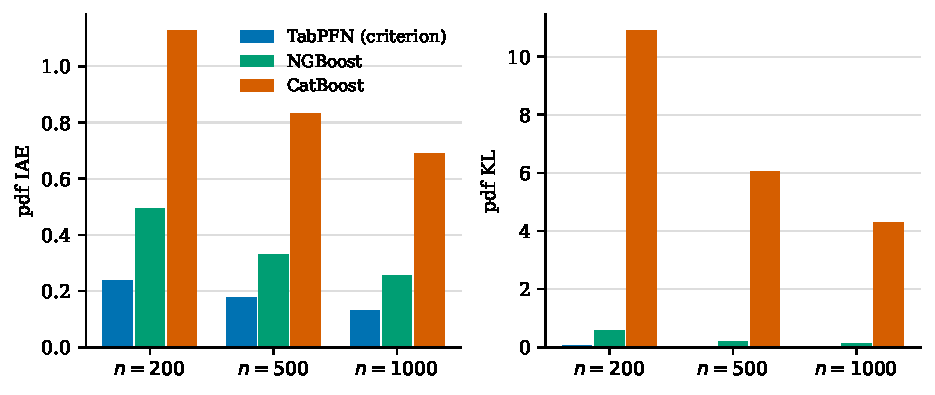
\includegraphics[width=\linewidth]{accuracy_by_n.pdf}
  \caption{Conditional-density accuracy by inner model and sample size:
  integrated absolute error (left) and Kullback--Leibler divergence
  (right) of the fitted pdf, averaged over families, $\tau(x)$ regimes,
  grid points and repetitions; error bars are $\pm 2$ standard errors over
  the $20$ repetitions. Colors follow the Okabe--Ito colorblind-safe
  palette.}
  \label{fig:accuracy-by-n}
\end{figure}

\begin{figure}[p]
  \centering
  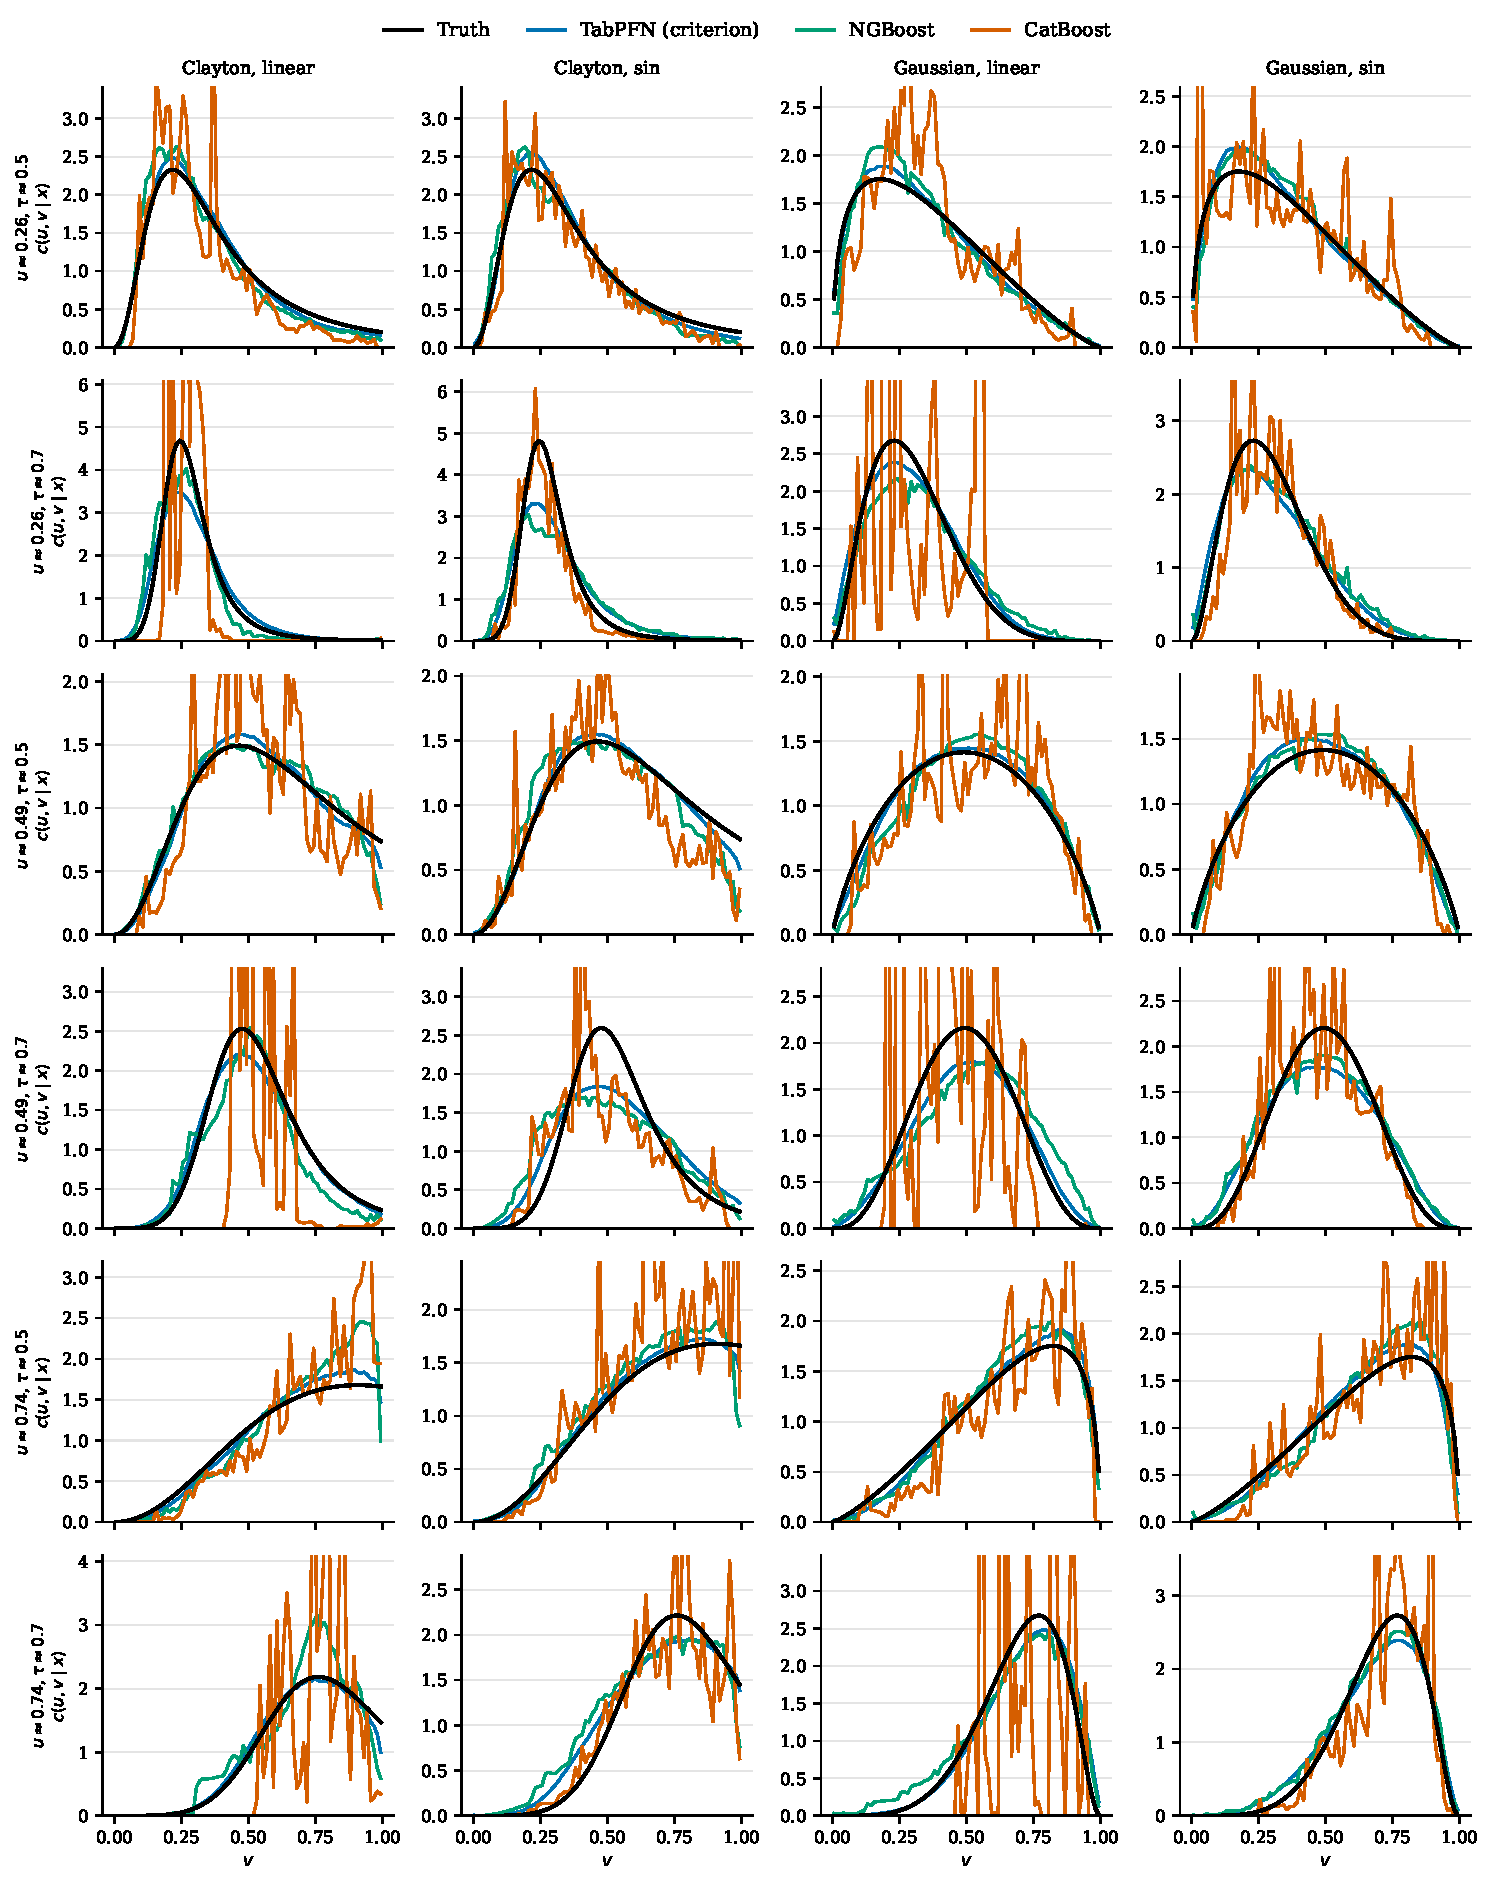
\includegraphics[width=\linewidth]{density_recovery_grid.pdf}
  \caption{Recovery of conditional copula density slices
  $c(u,\,v \mid x)$ by inner model, at $n=1000$ on an $80\times80$
  evaluation grid. Rows vary the fixed conditioning value
  ($u\approx0.25,0.5,0.75$) and the target dependence
  ($\tau(x)\approx0.5$, then $0.7$); columns vary the family and $\tau(x)$
  regime. Each panel plots the density against $v$, averaged over
  repetitions, with the exact copula in black. Each panel's $y$-axis is
  scaled to the truth and the two smooth estimators; where CatBoost's
  quantile-table reconstruction spikes above that range it is clipped.}
  \label{fig:density-recovery}
\end{figure}

\begin{figure}[t]
  \centering
  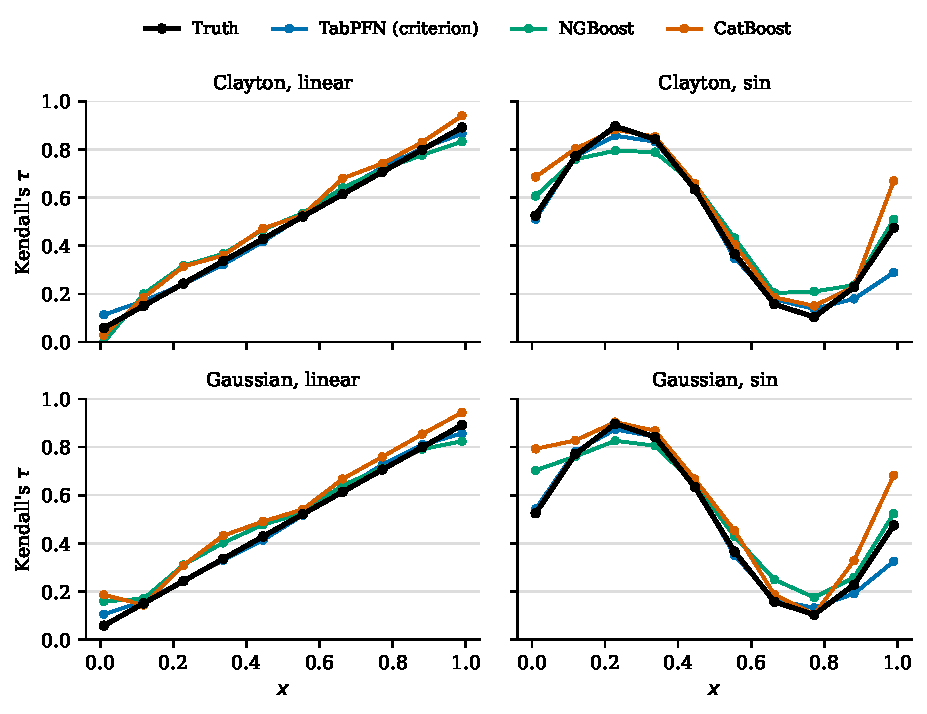
\includegraphics[width=\linewidth]{conditional_tau.pdf}
  \caption{Fitted conditional Kendall's tau $\widehat\tau(x)$ as a function
  of the covariate $x$, by inner model, for each family and $\tau(x)$
  regime at $n=1000$. The estimate at each $x$ is averaged over
  repetitions; the black curve is the target $\tau(x)$. Kendall's tau is
  computed from the fitted model by the inverse-Rosenblatt simulation
  recipe of Section~\ref{sec:kendall}.}
  \label{fig:conditional-tau}
\end{figure}

\section{Vine Simulation Study}
\label{sec:vine-study}

The bivariate study scores one conditional pair copula. The vine study
scores the construction the pair copulas are built for: a
$d$-dimensional conditional distribution
$f(\mathbf y \given x)$, $\mathbf y \in \R^d$, estimated as a regular vine
of NPCC pair copulas on top of NPCC margins. It asks two questions: how
much is lost when the vine structure is unknown, and how much is lost by
an estimator that ignores the covariate. The study runs in dimensions
$d \in \{3,5\}$, and it is implemented as \texttt{npcc-vinestudy},
configured by \texttt{configs/vine\_study.toml}.

\subsection{Data-Generating Process}

Each repetition draws one true model, specified in three parts.

\paragraph{Structure.} An R-vine structure $\mathcal V$ is drawn
uniformly over all regular vines on $d$ variables (Algorithm~13 of
Joe, 2014, as implemented by \texttt{RVineStructure.sample}). Tree
$t \in \{1,\ldots,d-1\}$ has $d-t$ edges, and an edge
$e = (a_e,b_e;D_e)$ has conditioning set $D_e$ with $|D_e| = t-1$.

\paragraph{Pair copulas.} Each edge independently draws a family,
uniformly from Clayton, Gumbel, Frank, Gaussian, and Joe, and a Kendall's
tau regime $\tau_e(\cdot)$, uniformly from the four conditional regimes
of Section~\ref{sec:scenarios} (linear, constant, sinusoidal,
quadratic). Dependence is weakened with the tree level: the regime is
mapped affinely from $[\tau_{\min},\tau_{\max}]$ onto
$[\tau_{\min},\tau_{\max}^{\,t}]$,
\begin{equation}
  \tau_{e}^{(t)}(x)
  =
  \tau_{\min}
  +
  \bigl(\tau_{\max}^{\,t}-\tau_{\min}\bigr)
  \frac{\tau_e(x)-\tau_{\min}}{\tau_{\max}-\tau_{\min}},
  \label{eq:tau-decay}
\end{equation}
with $(\tau_{\min},\tau_{\max}) = (0.05,0.70)$ as in the bivariate study.
Tree~1 therefore reproduces the bivariate regimes exactly, and the upper
ends of the bands of trees $1$ to $4$ are $0.70$, $0.49$, $0.34$, and
$0.24$. The family's parameter at $x$ is the one whose Kendall's tau equals
$\tau_e^{(t)}(x)$.

The pair copulas depend on the covariate $x$ but \emph{not} on the values
of their conditioning variables $\mathbf u_{D_e}$: on its own structure,
the truth satisfies the simplifying assumption given $x$. At any fixed $x$
it is therefore an ordinary parametric vine copula $c(\mathbf u \given x)$,
which supplies both exact sampling and exact densities.

\paragraph{Margins.} The margins are Gaussian with a location that moves
with the covariate,
\begin{equation}
  Y_j \given X = x \;\sim\; \mathcal N\bigl(\mu_j(x),\,1\bigr),
  \qquad
  \mu_j(x) = a_j\bigl(x-\tfrac12\bigr),
  \qquad
  a_j \sim \mathrm{Unif}[-2,2],
  \label{eq:vine-margins}
\end{equation}
independently for $j=1,\ldots,d$, so each marginal mean moves by up to one
standard deviation in either direction over the covariate range. By
Sklar's theorem the true joint density is
\begin{equation}
  f(\mathbf y \given x)
  =
  c\bigl(\mathbf u \given x\bigr)
  \prod_{j=1}^d \phi\bigl(y_j-\mu_j(x)\bigr),
  \qquad
  u_j = \Phi\bigl(y_j-\mu_j(x)\bigr),
  \label{eq:vine-joint}
\end{equation}
where $\phi$ and $\Phi$ denote the standard normal density and
distribution function. Gaussian margins have a second role: they keep $f$
bounded where the copula density $c$ has corner singularities, which is
what makes the integrated squared error of the joint density below finite
and estimable.

\paragraph{Training sample.} As in the bivariate study, the covariate is a
deterministic grid, $x_i$ equally spaced on $[0.01,0.99]$ for
$i=1,\ldots,n$. Each $\mathbf u_i$ is the inverse Rosenblatt transform of
independent uniforms under $c(\cdot \given x_i)$, and $\mathbf y_i$ is
obtained from Equation~\eqref{eq:vine-margins}. The sample sizes are
$n \in \{500,1000\}$, with five repetitions per $(d,n)$.

\subsection{Estimators}

Every estimator targets the joint density~\eqref{eq:vine-joint} on the
data scale. Each is fitted by the two-step method (inference functions for
margins): first the margins, then the vine copula on the estimated
probability integral transforms $\widehat u_{ij} = \widehat F_j(y_{ij}
\given x_i)$.

\begin{description}
  \item[\texttt{oracle}.] NPCC margins
    $\widehat F_j(\cdot \given x)$, fitted with the same inner model as
    the pairs but on the data scale (no support transform), and NPCC pair
    copulas on the \emph{true} structure $\mathcal V$. Since the truth is
    simplified on $\mathcal V$, every pair conditions on $x$ alone:
    $\widehat c_{a_e,b_e;D_e}(\cdot,\cdot \given x)$.
  \item[\texttt{random}.] The same margins, and NPCC pair copulas on a
    structure drawn uniformly at random and independently of the truth.
    On a wrong structure the true pair copulas generally depend on the
    conditioning values, so this vine is \emph{non-simplified}: an edge
    in tree $t \ge 2$ conditions on $(\mathbf u_{D_e}, x)$,
    $\widehat c_{a_e,b_e;D_e}(\cdot,\cdot \given \mathbf u_{D_e}, x)$. This
    is the realistic setting, in which the structure is unknown and the
    estimator has to make up for a wrong one.
  \item[\texttt{kde-tll}.] A covariate-blind baseline: univariate kernel
    density margins and nonparametric transformation local-likelihood
    (TLL) pair copulas from pyvinecopulib, on the true structure
    $\mathcal V$, with $x$ ignored throughout. Since it shares the
    oracle's structure, its gap to \texttt{oracle} prices the covariate
    alone.
\end{description}

The NPCC arms are run for each inner-model configuration in the grid;
the headline configuration is TabPFN (criterion head, v2.5) with the logit
transform on the pair copulas.

\subsection{Evaluation}

Scoring is done at fixed covariate values $x_k$, $k=1,\ldots,5$, equally
spaced on $[0.01,0.99]$. At each $x_k$, $m=1000$ test points
$\mathbf y^\ast_{k1},\ldots,\mathbf y^\ast_{km}$ are drawn from
$f(\cdot \given x_k)$, together with their true probability integral
transforms $\mathbf u^\ast_{kl}$. With $f$ the truth and $\widehat f$ an
estimate, three divergences between the two conditional densities of
$\mathbf y$ at the same $x_k$ are estimated by Monte Carlo under the
truth, writing $f = f(\mathbf y \given x_k)$ and
$\widehat f = \widehat f(\mathbf y \given x_k)$:
\begin{align}
  \mathrm{KL}(x_k)
  &= \int_{\R^d} f \log\frac{f}{\widehat f}\dd\mathbf y
  = \E_f\bigl[\log f - \log \widehat f\,\bigr]
  \approx \frac1m \sum_{l=1}^m
    \log\frac{f(\mathbf y^\ast_{kl} \given x_k)}
             {\widehat f(\mathbf y^\ast_{kl} \given x_k)},
  \label{eq:vine-kl}\\
  \mathrm{L1}(x_k)
  &= \int_{\R^d} \bigl|\widehat f - f\bigr|\dd\mathbf y
  = \E_f\Bigl|\frac{\widehat f}{f} - 1\Bigr|,
  \label{eq:vine-l1}\\
  \mathrm{ISE}(x_k)
  &= \int_{\R^d} \bigl(\widehat f - f\bigr)^2\dd\mathbf y
  = \E_f\Bigl[\frac{(\widehat f - f)^2}{f}\Bigr],
  \label{eq:vine-ise}
\end{align}
where $\E_f$ is the expectation over $\mathbf y \sim f(\cdot \given x_k)$,
and each expectation is estimated by the same average over the $m$ test
points. The integrals run over the response $\mathbf y$ alone: the
covariate is held at $x_k$ throughout, and no divergence is integrated
over $x$.

To separate copula error from margin error, the same KL and L1 are also
computed for the fitted vine copula alone, comparing
$\widehat c(\cdot \given x_k)$ with $c(\cdot \given x_k)$ as densities on
$(0,1)^d$, estimated at the true transforms $\mathbf u^\ast_{kl}$
(\texttt{KL\_copula}, \texttt{L1\_copula}). No copula-scale ISE is
reported: its Monte Carlo estimate divides by $c$, and the corner peaks of
$c$ make it too heavy-tailed to be informative.

Each metric is computed per $x_k$ and per repetition. The per-$x_k$ values
are reported directly (Figure~\ref{fig:vine-kl-by-x}), and the headline
summary is their average over $k$ within a repetition, for instance
$\overline{\mathrm{KL}} = \frac15\sum_{k=1}^5 \mathrm{KL}(x_k)$. That is an
average of fixed-$x$ divergences, not a divergence between densities
integrated over $x$. Across the $R = 20$ repetitions, the tables report
the mean and its standard error, $\mathrm{sd}/\sqrt R$.

\paragraph{Common random numbers.} The true model, the random structure of
the \texttt{random} arm, and the test points depend only on $(d,
\text{repetition})$; only the training sample also depends on $n$. Every
sample size in a repetition therefore faces the same truth and is scored
on the same test points, so differences across $n$ reflect estimation
alone. The arms also share them, so the difference between two arms is
reported paired within a repetition, which removes the between-truth
variation from its standard error.

\subsection{Results}
\label{sec:vine-results}

\providecommand{\se}[1]{{\scriptsize(#1)}}

All results are for the headline configuration, TabPFN (criterion head,
v2.5) with the logit transform on the pair copulas, over $R=20$
repetitions. Table~\ref{tab:vine-results} reports the $x$-averaged
divergences, and Figure~\ref{fig:vine-kl-by-x} shows the joint KL at each
evaluation covariate value. A split by copula family or tau regime, as in
the bivariate study, does not exist here: every true vine mixes families
and regimes across its edges, drawn afresh in each repetition.

\begin{figure}[!ht]
  \centering
  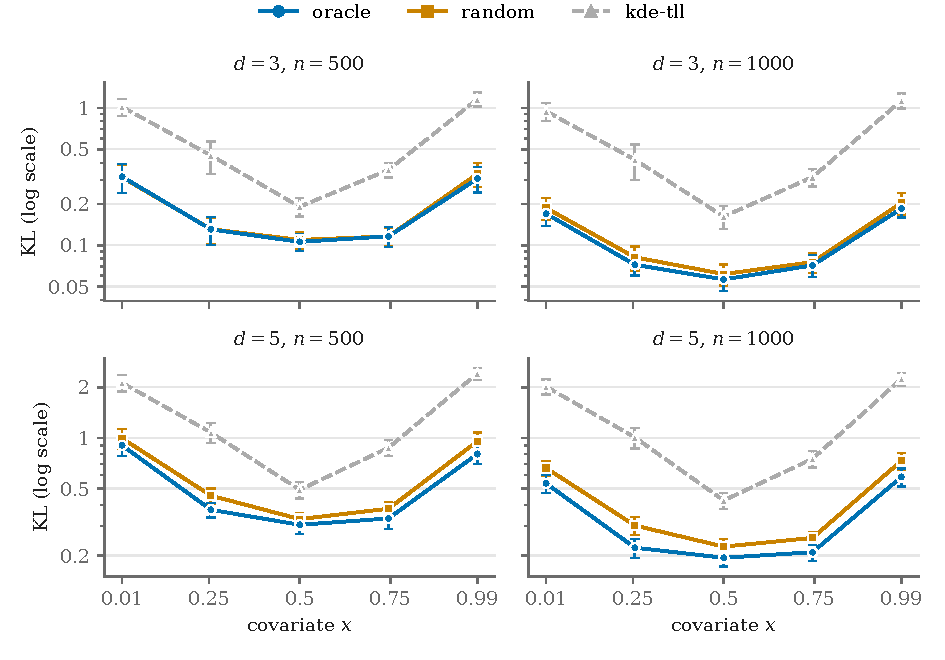
\includegraphics[width=\linewidth]{vine_kl_by_x.pdf}
  \caption{Vine study: joint-density KL divergence at each evaluation
  covariate value $x_k$, by dimension $d$, sample size $n$, and arm, as the
  mean over $20$ repetitions with $\pm 2$ standard errors. Log scale.}
  \label{fig:vine-kl-by-x}
\end{figure}

\begin{table}[h]
  \centering
  \footnotesize
  \setlength{\tabcolsep}{2.5pt}
  \begin{tabular}{llrrrrrrrr}
    \toprule
    & & \multicolumn{3}{c}{joint KL}
      & \multicolumn{3}{c}{copula KL}
      & \multicolumn{2}{c}{random $-$ oracle} \\
    \cmidrule(lr){3-5}\cmidrule(lr){6-8}\cmidrule(lr){9-10}
    $d$ & $n$ & oracle & random & kde-tll
      & oracle & random & kde-tll & KL & wins \\
    \midrule
    3 & 500  & 0.195 \se{0.015} & 0.200 \se{0.014} & 0.636 \se{0.029}
             & 0.157 \se{0.013} & 0.163 \se{0.013} & 0.392 \se{0.023}
             & 0.005 \se{0.005} & 13/20 \\
    3 & 1000 & 0.111 \se{0.006} & 0.122 \se{0.007} & 0.596 \se{0.030}
             & 0.087 \se{0.006} & 0.099 \se{0.007} & 0.371 \se{0.025}
             & 0.011 \se{0.004} & 13/20 \\
    5 & 500  & 0.543 \se{0.021} & 0.622 \se{0.023} & 1.397 \se{0.052}
             & 0.468 \se{0.023} & 0.555 \se{0.022} & 1.062 \se{0.050}
             & 0.079 \se{0.015} & 19/20 \\
    5 & 1000 & 0.350 \se{0.013} & 0.435 \se{0.010} & 1.289 \se{0.050}
             & 0.301 \se{0.016} & 0.382 \se{0.012} & 1.007 \se{0.048}
             & 0.085 \se{0.009} & 20/20 \\
    \bottomrule
  \end{tabular}
  \caption{Vine study: joint-density and copula-scale KL divergence, each
  the average over the five evaluation covariate values of a fixed-$x$
  divergence, as mean \se{standard error} over $20$ repetitions. The last
  two columns compare the two NPCC arms within each repetition, on common
  truths and test points: the mean paired difference in joint KL, and the
  number of repetitions in which the oracle's KL is the lower. Lower is
  better.}
  \label{tab:vine-results}
\end{table}

\paragraph{The covariate.} Both NPCC arms improve on the covariate-blind
baseline by a wide margin, and in every one of the $80$ repetitions: the
joint KL of \texttt{kde-tll} is two to five and a half times theirs, and it barely
improves with $n$, since more data cannot make up for a model that ignores
$x$. Figure~\ref{fig:vine-kl-by-x} locates the gap: it is widest at the
ends of the covariate range, where the tau regimes and the marginal
locations are furthest from their averages. At $d=3$ the baseline's KL is
about $1.0$ to $1.1$ at $x \in \{0.01,0.99\}$ against $0.18$ at $x=0.5$,
while the oracle's is $0.24$ and $0.08$.

\paragraph{The structure.} At $d=3$ a random structure costs little: the
paired difference in joint KL, as mean $\pm$ one standard error, is
$0.005 \pm 0.005$ at $n=500$,
indistinguishable from zero, and $0.011 \pm 0.004$ at $n=1000$, small but
detectable. A three-dimensional vine has only three possible structures,
and a non-simplified NPCC absorbs most of a wrong one through its
conditioning. At $d=5$ the cost is clear: about $0.08$ in joint KL, some
$15$ to $25\%$ of the oracle's, with the oracle ahead in $39$ of $40$
repetitions. Doubling $n$ reduces the NPCC KL by $30$ to $43\%$ in every
case.

\paragraph{Copula and margins.} The copula-scale KL accounts for most of
the joint KL. For the NPCC arms the difference, a proxy for the margins'
share, is $0.02$ to $0.08$; for \texttt{kde-tll} it is $0.22$ to $0.34$,
the price of margins that ignore the location shift in $x$. The
integrated squared error of the joint density tells the same story: in
units of $10^{-2}$, it is $1.06 \pm 0.09$, $1.10 \pm 0.10$, and
$3.13 \pm 0.17$ for oracle, random, and \texttt{kde-tll} at $d=3$,
$n=500$, and $0.72 \pm 0.07$, $0.82 \pm 0.08$, and $1.79 \pm 0.13$ at
$d=5$, $n=1000$.

\paragraph{Cost.} On the study GPU box, the median fit of one NPCC vine
distribution takes $3.5$~s at $d=3$ and $10$~s at $d=5$, and evaluating it
at the $5000$ test points takes about $25$ and $82$~s. The TLL baseline
takes a fraction of a second for both. The machine was shared with another
study during part of the run, so these times are indicative.

\section{Implementation Correspondence}

\begin{table}[h]
  \centering
  \begin{tabular}{ll}
    \toprule
    Mathematical object & Implementation \\
    \midrule
    Symmetric estimator in Equation~\eqref{eq:symmetric-density}
      & \texttt{RosenblattBicop} \\
    Criterion predictive distribution
      & \texttt{TabPFNCriterionBackend} \\
    Quantile predictive distribution
      & \texttt{TabPFNQuantileBackend} \\
    Shared support transforms
      & \texttt{ConditionalMargin} \\
    Sinkhorn projection
      & \texttt{sinkhorn\_iters} \\
    \bottomrule
  \end{tabular}
\end{table}

\end{document}
